\documentclass[
	aspectratio=169, % default is 43
	8pt, % font size, default is 11pt
	handout, % handout mode without animations, comment out to add animations
]{beamer}
\def\university{}

\documentclass[
	aspectratio=169, % default is 43
	8pt, % font size, default is 11pt
	handout, % handout mode without animations, comment out to add animations
]{beamer}

\usepackage{../template/beamerthemeuulm} % use the inofficial uulm beamer theme
\setfaculty{infIngPsy} % set the color scheme for your faculty here [med/infIngPsy/math/nat]

% requires symbolic links
% git clone git@github.com:SoftVarE-Group/SlideTemplate.git C:\Users\...\SlideTemplate
% mklink /J template C:\Users\...\SlideTemplate
% git clone git@spgit.informatik.uni-ulm.de:thuem/slides.git C:\Users\...\ThomasSlides
% mklink /J thomasslides C:\Users\...\ThomasSlides
\graphicspath{{../template/pics/logos}{../template/pics/nature}{../template/pics/uulm}{../thomasslides/}{../pics/people/}{../pics/xkcd/}}

%\usepackage[ngerman]{babel} % use this line for slides in German
%\recordingtrue % special recording mode for use with a greenscreen, gives you space to show yourself in a layer in front of the slides, has no effect in the handout mode

\title{Software Product Lines} % short title is used for the slide footer but optional

% LINKED LITERATURE

\newcommand{\ludewiglichter}{\href{https://learning.oreilly.com/library/view/-/9781457184932/?ar}{Ludewig and Lichter}}
\newcommand{\seeconomics}{\href{https://rds-ulm.ibs-bw.de/link?kid=027381854}{SE Economics}}
\newcommand{\sommervillelink}[1]{\href{https://ulm.ibs-bw.de/aDISWeb/app?service=direct/0/Home/$DirectLink\&sp=SOPAC00\&sp=SAKSWB-IdNr1615420983}{#1}}
\newcommand{\sommerville}{\sommervillelink{Sommerville}}
\newcommand{\thehumbleprogrammer}{\href{https://dl.acm.org/doi/10.1145/1283920.1283927}{The Humble Programmer}}
\newcommand{\thepragmaticprogrammer}{\href{https://learning.oreilly.com/library/view/the-pragmatic-programmer/9780135956977/}{The Pragmatic Programmer}}

% TYPICAL COMMANDS FOR LECTURES

\renewcommand{\emph}[1]{{\color{blue}\textbf{#1}}}

\newcommand{\deutsch}[1]{{\color{blue}(#1)}}
\newcommand{\deutschertitel}[1]{{\tiny\deutsch{#1}}}

\newcommand{\mycite}[1]{``#1''}
\newcommand{\mytitlesource}[1]{{\tiny\normalfont\mbox{[#1]}}}
\newcommand{\mysource}[1]{\ifthenelse{\equal{#1}{}}{}{\phantom{.}~\hfill~\mytitlesource{#1}}}

\newcommand{\todo}[1]{{\color{red}\textbf{[#1]}}}
\newcommand{\fodo}[1]{\todo{\footnote{\todo{#1}}}}
\newcommand{\todots}{\todo{\ldots}}

% IMPORTED PACKAGES

%\usepackage{adjustbox} % used for partofpage
%\usepackage{tcolorbox} % used for mydefinition, mynote, myexample
\usepackage{multicol} % used temporarily for the lecture overview
\usepackage{mathtools} % required for absolute value in modeling lecture

% COMMANDS TO LAYOUT AND ANNIMATE SLIDES

\newcommand{\lessonslearned}[3]{
	\subsection{Summary}
	\begin{frame}{\insertsection -- \insertsubsection}
		\leftorright{
			\mydefinition{Lessons Learned}{
				\begin{itemize}
					#1
				\end{itemize}
			}
			\mynote{Further Reading}{
				\small % references take space, can be a little smaller
				\begin{itemize}
					#2
				\end{itemize}
			}
		}{
			\myexample{Practice}{
				#3
			}
		}
	\end{frame}
}

% TODO temporary hack to layout the slide overview in two colums
\renewcommand{\lectureoverview}{
%	\section*{Overview}
%	\subsection*{Overview}
	\begin{frame}{\insertsubtitle}
		\begin{multicols}{2}
			\tableofcontents
		\end{multicols}
	\end{frame}
}

\renewcommandx{\maketitle}[2][1=apr21-o25a,2=150]{
    {
	\usebackgroundtemplate{} % TODO temporary hack to enable missing pictures at title slide
	%\ifx {#1} \empty \else {\usebackgroundtemplate{\includegraphics[trim=0 0 0 #2,clip,width=\paperwidth]{#1}}} \fi     
	%\usebackgroundtemplate{\includegraphics[trim=0 0 0 #2,clip,width=\paperwidth]{#1}}
    \begin{frame}[plain]
        \vskip0pt plus 1filll
        \begin{beamercolorbox}[wd=\paperwidth,ht=4.5ex,dp=2ex,right]{titlebox}
            \LARGE\textbf{\inserttitle}\hspace*{20pt}
        \end{beamercolorbox}%
        \nointerlineskip%
        \begin{beamercolorbox}[wd=\paperwidth,ht=2.25ex,dp=1ex,right]{subtitlebox}
            \small 
            \ifx \insertsubtitle \empty \else \insertsubtitle\ $\vert$ \fi
            \insertauthor\
            \ifx \insertdate \empty \else $\vert$ \insertdate \fi
            \hspace*{20pt}
        \end{beamercolorbox}%
        \nointerlineskip%
        \begin{beamercolorbox}[wd=\paperwidth,ht=4.5ex,dp=2ex,left]{logobox}
            \centering
            \vspace{-1ex}
            \hspace{10pt}
            \includegraphics[height=4.5ex]{sp} % SPECIFY INSTITUTE LOGO HERE
            \hfill
            \includegraphics[height=4.5ex]{uulm}
            \hspace{10pt}
        \end{beamercolorbox}%
    \end{frame}
    }  
}

%
%\newcommand{\onlyleft}[1]{
%	\halfpage{#1}
%}
%
%\newcommand{\onlyright}[1]{
%	~\hfill
%	\halfpage{#1}
%}
%
%\newcommand{\leftorright}[2]{
%	\uncover<1>{\halfpage{#1}}
%	\hfill
%	\uncover<3->{\halfpage{#2}}
%}
%
%\newcommand{\rightorleft}[2]{
%	\uncover<3->{\halfpage{#1}}
%	\hfill
%	\uncover<1>{\halfpage{#2}}
%}
%
%\newcommand{\leftthenright}[2]{
%	\halfpage{#1}
%	\hfill\pause
%	\halfpage{#2}
%}
%
%\newcommand{\leftandright}[2]{
%	\halfpage{#1}
%	\hfill
%	\halfpage{#2}
%}
%
%\newcommand{\leftmiddleandright}[3]{
%	\thirdpage{#1}
%	\hfill
%	\thirdpage{#2}
%	\hfill
%	\thirdpage{#3}
%}
%
%\newcommand{\leftmiddleorright}[3]{
%	\uncover<1>{\thirdpage{#1}}
%	\hfill
%	\uncover<3>{\thirdpage{#2}}
%	\hfill
%	\uncover<5->{\thirdpage{#3}}
%}
%
%\newcommand{\halfpage}[1]{\partofpage{48}{#1}}
%
%\newcommand{\thirdpage}[1]{\partofpage{31}{#1}}
%
%\newcommand{\partofpage}[2]{
%	\adjustbox{valign=t}{\begin{minipage}{0.#1\textwidth}
%			\begin{flushleft}
%				#2
%			\end{flushleft}
%	\end{minipage}}
%}
%
%\newcommand{\mydefinition}[2]{
%	\begin{tcolorbox}[title=#1,colback=orange!10,colframe=orange!30,coltitle=black,fonttitle=\bfseries,left=1mm,right=1mm,top=1mm,bottom=1mm]
%		\begin{flushleft}
%			#2
%		\end{flushleft}
%	\end{tcolorbox}
%}
%
%\newcommand{\mydefinitiontight}[2]{
%	\begin{tcolorbox}[title=#1,colback=white,colframe=orange!30,coltitle=black,fonttitle=\bfseries,left=0mm,right=0mm,top=0mm,bottom=0mm]
%		\begin{flushleft}
%			#2
%		\end{flushleft}
%	\end{tcolorbox}
%}
%
%\newcommand{\mynote}[2]{
%	\begin{tcolorbox}[title=#1,colback=red!10,colframe=red!30,coltitle=black,fonttitle=\bfseries,left=1mm,right=1mm,top=1mm,bottom=1mm]
%		\begin{flushleft}
%			#2
%		\end{flushleft}
%	\end{tcolorbox}
%}
%
%\newcommand{\myexample}[2]{
%	\begin{tcolorbox}[title=#1,colback=blue!10,colframe=blue!30,coltitle=black,fonttitle=\bfseries,left=1mm,right=1mm,top=1mm,bottom=1mm]
%		\begin{flushleft}
%			#2
%		\end{flushleft}
%	\end{tcolorbox}
%}
%
%\newcommand{\myexampletight}[2]{
%	\begin{tcolorbox}[title=#1,colback=white,colframe=blue!30,coltitle=black,fonttitle=\bfseries,left=0mm,right=0mm,top=0mm,bottom=0mm]
%		\begin{flushleft}
%			#2
%		\end{flushleft}
%	\end{tcolorbox}
%}

\subtitle{7. Languages for Features}
\author{Timo Kehrer, Thomas Thüm, Elias Kuiter}

\begin{document}

\mode<handout>{\contentoverview}

\mode<beamer>{
	\ifdefined\thepicture
		\maketitle[\thepicture][\thepictureoffset]
	\else
		\maketitle[]
	\fi
}

% shared slide content

% introduced: 02a-configuration
% reused: 03a-intro
\newcommand{\frameImplementSPLs}{
	\begin{mycolumns}[widths={45},animation=none]
		\pic[width=\linewidth]{metaproduct2}
	\mynextcolumn
		\begin{note}{Key Issues}
			\begin{itemize}
			\item Systematic reuse of implementation artifacts
			\item Explicit handling of variability
			\end{itemize}
		\end{note}
		\uncover<2->{\begin{definition}{Variability\mysource{\fospl\mypage{48}}}
			\mycite{\emph{Variability} is the ability to derive different products from a common set of artifacts.}
		\end{definition}}
		~
		\uncover<3->{\begin{note}{Variability-Intensive System}
			Any software product line is a variability-intensive system. % TODO Timo: do we really need this term? where does this definition come from?
		\end{note}}
	\end{mycolumns}
}

% introduced: 02a-configuration
% reused: 02b-implementation, 03a-intro
\newcommand{\frameVariabilityAndBindingTimes}{
	\begin{mycolumns}[widths={55},animation=none]
		\begin{definition}{Binding Time \deutsch{Bindungszeitpunkt}\mysource{\fospl\mypage{48}}}
			\begin{itemize}
				\item Variability offers choices
				\item Derivation of a product requires to make decisions (aka. binding)
				\item Decisions may be bound at different binding times
			\end{itemize}
		\end{definition}
		~
		\uncover<2->{\begin{note}{When? By whom? How?}
			\lectureruntime\parta: \emph{when} and \emph{by whom}

			\lectureruntime\partb: \emph{how}
		\end{note}}
	\mynextcolumn
		\pic[width=\linewidth]{metaproduct2}
	\end{mycolumns}
}

% introduced: 03a-intro
% reused: 03a-intro
\newcommand{\frameRuntimeVariabilityProblems}{
	\begin{note}{Problems of Runtime Variability}
		{\bf Conditional Statements:}
		\begin{itemize}
			\item Code scattering, tangling, and replication
		\end{itemize}
		{\bf Design Patterns for Variability:}
		\begin{itemize}
			\item Trade-offs and potential negative side effects
			\item Constraints that may restrict their usage
		\end{itemize}
		{\bf In General:}
		\begin{itemize}
			\item Variable parts are always delivered
			\item Not well-suited for compile-time binding
		\end{itemize}
	\end{note}
}

% introduced: 03a-intro
% reused: 03a-intro
\newcommand{\frameSoftwareConfigurationManagement}{
	\begin{mycolumns}
		\begin{definition}{Software Configuration Management} % TODO source missing
			Policies, processes, and tools for managing evolving software systems:
			\begin{itemize}
				\item Version control
				\item System building
				\item Release management
				\item Change management
				\item Collaborative work
			\end{itemize}
		\end{definition}
	\mynextcolumn
		\begin{note}{No Software Configuration Management}
			\lecturecloneandown\parta: Ad-Hoc Clone-and-Own

			aka.\ unmanaged clone-and-own
		\end{note}
		\begin{note}{Version Control}
			\lecturecloneandown\partb: Clone-and-Own with Version Control

			instance of managed clone-and-own
		\end{note}
		\begin{note}{System Building}
			\lecturecloneandown\partc: Clone-and-Own with Build Systems

			instance of managed clone-and-own
		\end{note}
	\end{mycolumns}
}


\section{Limits of Object-Orientation}
% of Classical Programming Paradigms
% of Teachniques for Application Software

%\subsection{Expression Problem? Preplanning? Tyrany}
%\subsection{Multiple Inheritance}
%\subsection{Mixins}
%\subsection{Design Patterns}
%\subsection{Default Methods}
%\subsection{\ldots}

\subsection{Recap: Object-Oriented Key Concepts}

\begin{frame}{Recap: Object-Oriented Key Concepts}
	\leftorright{
		\mydefinition{Encapsulation}{Abstraction \& Information Hiding}		
		\mydefinition{Composition}{Nested objects}	
		\mydefinition{Message Passing}{Delegating responsibility}
		\mydefinition{Distribution of Responsibility}{Separation of concerns}	
		\mydefinition{Inheritance}{Conceptual hierarchy, polymorphism, reuse}
	}{
		\pic[width=0.8\linewidth]{oo-concepts-illustration} % was illustriert was? warum ist square kein rectangle?
	}
\end{frame}

\begin{frame}{Recap: Design Patterns (for Variability) \mytitlesource{\gof}}
	\leftorright{
		\vspace{-10mm}
		\mynote{Design patterns \deutsch{Entwurfsmuster}}{
			\begin{itemize}
				\item Document common solutions to concrete yet frequently occurring design problems.
				\item Suggest a concrete implementation for a specific object-oriented programming problem.
			\end{itemize}
		}		
		\mynote{Design patterns for variability}{
			\begin{itemize}
				\item Many Gang of Four (GoF) design patterns for designing software around stable abstractions and interchangeable (i.e., variable) parts, e.g.
				\begin{itemize}
					\item Template Method
					\item Abstract Factory
					\item Decorator
				\end{itemize}
			\end{itemize}
		}				
	}{
		\pic[width=\linewidth]{gof}
	}
\end{frame}

\begin{frame}{Recap: Modularity - Components, Services, and Frameworks}
	\begin{mycolumns}[widths={40,60},animation=none]
		\myexample{Component-/Service-Based SPLs}{
			\pic[width=.23\linewidth,height=1.0cm]{lego_components} 
				\vspace*{\fill}
					$+$ 
				\vspace*{\fill}	
			\pic[width=.23\linewidth,height=1.0cm]{lego_orchestration}
				\vspace*{\fill}
					$=$ 
				\vspace*{\fill}	
			\pic[width=.3\linewidth,height=1.0cm]{lego_product}
		}		
		\myexample{Specification of ``composition'' (glue code, orchestration)}{
			\centering
			\pic[width=.45\linewidth,height=1.7cm]{lego_orchestration}				
		}				
	\mynextcolumn		
		\myexample{Framework-Based SPLs}{
			\pic[width=.31\linewidth,height=1.75cm]{lego_product_partial} 
				\vspace*{\fill}
					$+$ 
				\vspace*{\fill}	
			\pic[width=.27\linewidth,height=1.75cm]{lego_components}
				\vspace*{\fill}
					$=$ 
				\vspace*{\fill}	
			\pic[width=.31\linewidth,height=1.75cm]{lego_product}
		}	
		\mynote{}{
			Neither glue code nor service composition required.
		}			
	\end{mycolumns}	
\end{frame}

\begin{frame}[fragile]{Recap: Extending Basic Graphs by Plug-Ins?}
	\tiny\begin{mycolumns}[columns=2,widths={50,50}]
\begin{codetight}{}
public class Graph {
	@private List<GraphPlugin> plugins = new ArrayList<GraphPlugin>();@
	// ...	
	@public void registerPlugin(GraphPlugin p){
		plugins.add(p);
	}@
	public void addNode(int id, Color c){
		Node n = new Node(id);
		@notifyAdd(n, c);@
		nodes.add(n);
	}
	public void print() {
		for (Node n : nodes) {
			@notifyPrint(n);@
			// ...
		}
		// ...
	}
	@private void notifyAdd(Node n, Color c) {
		for (GraphPlugin p : plugins) {
			p.aboutToAdd(n, c);
		}
	}
	private void notifyPrint(Node n) {
		for (GraphPlugin p : plugins) {
			p.aboutToPrint(n);
		}
	}@
	// ...
}
\end{codetight}
		\mynextcolumn
\begin{codetight}{}
public interface GraphPlugin {
	public void aboutToAdd(Node n, Color c);
	public void aboutToAdd(Edge e, Weight w);
	public void aboutToPrint(Node n);
	public void aboutToPrint(Edge e);
}
\end{codetight}
\begin{codetight}{}
public class ColorPlugin implements GraphPlugin {
	private Map<Node, Color> map = new HashMap<Node, Color>();

	public void aboutToAdd(Node n, Color c) {
		map.put(n, c);
	}
	
	public void aboutToAdd(Edge e, Weight w) {
		~// do nothing~
	}
	
	public void aboutToPrint(Node n) {
		Color c = map.get(n);
		Color.setDisplayColor(c);
	}
	
	public void aboutToPrint(Edge e) {
		~// do nothing~
	}
}
\end{codetight}
	\end{mycolumns}
\end{frame}

\begin{frame}{Recap: Challenges and Problems}
	\begin{mycolumns}[widths={50,50}]
		\myexample{}{
			In our example, we can observe that:
			\begin{itemize}
				\item There are lots of empty methods in the ColorPlugin 
				\item The framework consults all registered plug-ins before printing a node or edge
			\end{itemize}
		}		
		\mydefinition{General Challenge: Cross-cutting Concerns}{
			Implementing cross-cutting concerns as plug-ins 
			\begin{itemize}				
				\item typically leads to huge interfaces, large parts of which are irrelevant for a dedicated plug-in 
				\item causes lots of communication overhead between plug-ins and framework
			\end{itemize}
		}
	\mynextcolumn
		\myexample{}{
			If we were not familiar with our graph library, would we anticipate that:
			\begin{itemize}
				\item Colors and weights should be part of the Plugin interface?
				\item Every plug-in needs to be notified that the framework is about to print a node or edge? 
			\end{itemize}
		}
		\mydefinition{Generally known as Preplanning Problem}{
			\begin{itemize}
				\item Hard to identify and foresee the relevant hot spots and nature of extensions
				\item Developing a framework needs lots of expertise and excellent domain knowledge 
			\end{itemize}
		}	
	\end{mycolumns}
\end{frame}

\subsection{Preplanning Problem}

\begin{frame}{Preplanning Problem}
	\begin{mycolumns}[widths={45,55},animation=none]
		\mynote{Components, Services, and Frameworks}{
			Extensions are not possible ad-hoc, but must be foreseen and planned in advance:
			\begin{itemize}
				\item Frameworks: Hot spots / extension points
				\item Components/services: Provided and required interfaces 
			\end{itemize}
			\emph{$\Rightarrow$ No modular extension without a suitable extension point / interface!}
		}
	\mynextcolumn
		\mynote{And classical OO language concepts?}{
			Subtyping and polymorphism allow for ad-hoc extensions to some extent, but:
			\begin{itemize}
				\item Often, client code and/or basic implementation need to be adapted, too (non-modular)
				\item Limited flexibility of inheritance hierarchies (no ``mix and match'' supporting arbitrary feature combinations)
			\end{itemize}
			\emph{$\Rightarrow$ No variable extension without loosing modularity!}
		}
	\end{mycolumns}
\end{frame}

\subsection{Crosscutting Concerns}

\begin{frame}{Crosscutting Concerns}
	\begin{mycolumns}[widths={50,50},animation=none]
		\mydefinition{Concern \mysource{\fospl\mypages{55}}}{
			A concern is an area of interest or focus in a system, and features are the concerns of primary interest in product-line engineering.
		}
	\mynextcolumn
		\mydefinition{Crosscutting (Concern) \mysource{\fospl\mypages{55}}}{
			Crosscutting is a structural relationship between the representations of two concerns. 
			It is an alternative to hierarchical and block structure.
		}
	\end{mycolumns}
\end{frame}

\subsection{Tyranny of the Dominant Decomposition}

\begin{frame}{Tyranny of the Dominant Decomposition}
	\begin{mycolumns}[widths={50,50},animation=none]
		\mydefinition{Tyranny of the Dominant Decomposition}{
			\begin{itemize}
				\item Many concerns can be modularized, but not always at the same time.
				\item Developers choose a decomposition, but some other concerns cut across.
				\item Simultaneous modularization along different dimensions is not possible.
			\end{itemize}
		}
	\mynextcolumn
		\mynote{}{
			Crosscutting concerns are inherently difficult to separate using traditional mechanisms.
			\begin{itemize}
				\item Logging: Each time a method is called.
				\item Chaching/Pooling: Each time an object is created.
				\item Synchronization/Locking: Extension of many methods with lock/unlock calls.
			\end{itemize}
			Features in a software product line are often crosscutting (e.g., color and weight in our graph example).
		}
	\end{mycolumns}
\end{frame}

\begin{frame}{Another Example: Arithmetic Expressions}
	\begin{mycolumns}[widths={50,50},animation=none]
		\myexample{}{
			\begin{itemize}
				\item Arithemtic expressions are stored in a tree structure.
				\item Terms (i.e., sub-trees) can be evaluated and printed.
			\end{itemize}
		}
		\mynote{Question}{
			How to separate data structures and operations such that both can be extended independently of each other?
		}
	\mynextcolumn
		\myexampletight{}{
			\centering
			\pic[width=0.5\linewidth]{expressions}
		}
	\end{mycolumns}
\end{frame}

\begin{frame}{Arithmetic Expressions - Data-centric Implementation}
	\begin{mycolumns}[widths={40,60},animation=none]
		\mydefinition{Implementation Variant 1: Data-centric}{
			\begin{itemize}
				\item Recursive class structure (composite pattern)
				\item For each operation (eval, print, ...) there is a dedicated method in each class (Number, Plus, ...) 				
			\end{itemize}
		}
		\mynote{Terms are modular, but...}{
			\begin{itemize}
				\item New operations, e.g. drawTree or simplify, cannot simply be added
				\item All existing classes must be adjusted!
				\item Operations cut across the expressions.
			\end{itemize}
		}
	\mynextcolumn
		\myexampletight{}{
			\pic[width=\linewidth]{data_centered}
		}
	\end{mycolumns}
\end{frame}

\begin{frame}{Arithmetic Expressions - Operation-centric Implementation}
	\begin{mycolumns}[widths={40,60},animation=none]
		\mydefinition{Implementation Variant 2: Operation-centric}{
			\begin{itemize}
				\item Just a single accept method per class (visitor pattern).
				\item Each operation is implemented by a dedicated visitor.				
			\end{itemize}
		}
		\mynote{Operations are modular, but...}{
			\begin{itemize}
				\item New expressions, e.g. Min or Power, cannot simply be added
				\item For each new class, all visitor classes must be adjusted
				\item Expressions cut across operations
			\end{itemize}
		}
	\mynextcolumn
		\myexampletight{}{
			\pic[width=\linewidth]{method_centered}
		}
	\end{mycolumns}
\end{frame}

\begin{frame}{Lessons Learned from the Simple Example}
	\mynote{}{
		Hardly impossible to modularize expressions and operations at the same time!
	}
	\begin{mycolumns}[widths={50,50},animation=none]
		\mynote{Data-centric approach}{
			\begin{itemize}
				\item New expressions can be added directly: modular.
				\item New operations must be added to all classes: not modular.
			\end{itemize}
		}
	\mynextcolumn
		\mynote{Method-centric approach}{
			\begin{itemize}
				\item New operations can be added as another visitor: modular.
				\item For new expressions, all existing visitors must be extended: not modular.
			\end{itemize}
		}			
	\end{mycolumns}
\end{frame}

\lessonslearned{
	\item Important problems of previous approaches
	\begin{itemize}
		\item Inflexible inheritance hierarchies (especially with runtime variability, frameworks, components, services)
		\item Feature traceability (especially with runtime variability, branches, build systems, preprocessors)	
		\item Preplanning problem (esp. with frameworks, components, services)
		\item Cross-cutting issues (esp. with frameworks, components, services)
	\end{itemize}
}{
	\item s.\ previous lectures
}{
	Looking at our graph implementation serving as running example throughout the course: 
	\begin{itemize}
		\item Which concern is the dominant one regarding modular decomposition? %data structures
		\item What are crosscutting concerns? %color, weight, ...
		\item Could you rewrite the design to come up with a different decomposition?
	\end{itemize}
}

\sectionend

\section{Feature-Oriented Programming}

%\subsection{Delta-Oriented Programming}
% see spl07b.tex in old Latex slides (slides created by Thomas Thuem)

\subsection{Motivation}

\begin{frame}{Motivation}
	\begin{mycolumns}[widths={50,50},animation=none]
		\myexampletight{Modularization of Cross-Cutting Concerns}{
			\centering
			\pic[width=1.0\linewidth]{aop-motivation-1}
		}
		\myexample{Feature Traceability}{
			find feature 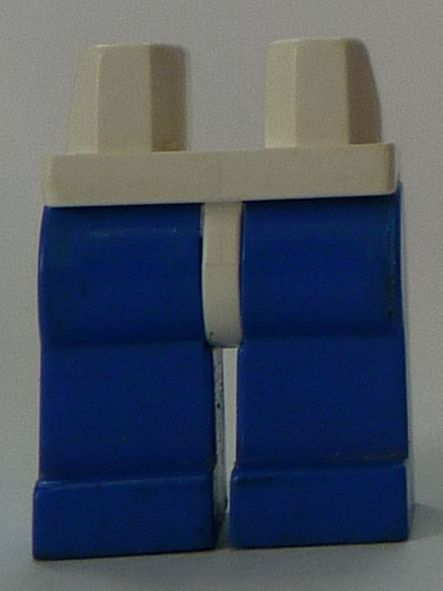
\includegraphics[width=.15\linewidth]{pants-blue} in product 
\includegraphics[width=.15\linewidth]{230}
		}
	\mynextcolumn
		\myexampletight{Flexible Extension / Minimal Preplanning}{
			\centering
			\pic[width=1.0\linewidth]{aop-motivation-2}
		}
		
		~
		
		\mynote{}{
			Achieving all this requires novel implementation techniques that overcome the limitations of classical object-oriented paradigms.
		}
	\end{mycolumns}
\end{frame}

\subsection{Feature Modules}

\begin{frame}{Background: Collaboration-Based Design} % TODO: is this original source ? \mytitlesource{Reenskaug et al.\ 1992}
	\begin{mycolumns}[widths={50,50},animation=none]
		\mydefinition{Inspiration: Collaborations in the Real World}{
			\begin{itemize}
				\item People collaborate to achieve a common goal.
				\item A collaboration typically comprises several persons playing different roles.
				\item Persons may play multiple roles by participating in different collaborations.
			\end{itemize}
		}
		\myexample{Mentor-Student Collaboration}{
			\begin{itemize}
				\item A person in the role of a mentor has responsibilities to instruct students on certain topics.
				\item A person in the role of a student has responsibilities to study the offered material.
			\end{itemize}
		}
	\mynextcolumn
		\mydefinition{Collaborations in Java \mysource{\fospl\mypages{131}}}{
			\begin{itemize}
				\item A \emph{collaboration} is a set of interacting classes, each class playing a distinct role, to achieve a certain function or capability. 
				\item A \emph{role} defines the responsibilities a class takes in a collaboration.
			\end{itemize}
		}
		\mynote{}{
			\begin{itemize}
				\item Different classes play different roles within a collaboration.
				\item A class plays different roles in different collaborations.
				\item A role encapsulates the behavior/functionality of a class relevant to a collaboration.
			\end{itemize}
		}
	\end{mycolumns}
\end{frame}

\begin{frame}{Example: Collaborations, Classes and Roles}
	\myexampletight{}{
		\centering
		\pic[width=1.0\linewidth]{collaborations}
	}
\end{frame}

\subsection{Feature Composition}

\begin{frame}{Feature Modules and Feature Module Composition}
	\begin{mycolumns}[widths={65,35},animation=none]
		\mydefinition{Feature Modules}{
			\begin{itemize}
				\item Each collaboration maps to a feature and is called a feature module (or layer).
				\item Feature modules may refine a base implementation by adding new elements or by modifying and extending existing ones.
			\end{itemize}
		}
	\mynextcolumn
		\mydefinition{Feature Module Composition}{
			Selected feature modules may be superimposed by lining-up classes according to the roles they play.
		}
	\end{mycolumns}
	\myexampletight{}{
		\centering
		\pic[width=0.95\linewidth]{feature-modules}
	}
\end{frame}

\begin{frame}{Feature Modules and Feature Module Composition}
	\mynote{Open Questions}{
		\begin{itemize}
			\item How to bundle classes to feature modules and specify their refinements?
			\item How to handle refinements during composition of feature modules?
		\end{itemize}
	}
	\myexampletight{}{
		\centering
		\pic[width=1.0\linewidth]{feature-modules}
	}
\end{frame}

\subsection{FOP in Java}

\begin{frame}{Jak: A Java Extension for Feature-Oriented Programming \mytitlesource{Batory et al.\ 2004}}
	\begin{mycolumns}[widths={50,50},animation=none]
		\mydefinition{Layers}{
			\begin{itemize}
				\item The keyword layer denotes the feature a class belongs to.
				\item A layer is a set of files that define a feature of an application.
			\end{itemize}
		}
		\mydefinition{Class Refinement}{
			A class refinement (keyword refines) can add new members to a class and extend existing methods. 
		}
		\mydefinition{Composer}{
			\begin{itemize}
				\item AHEAD (Algebraic Hierarchical Equations for Application Design) + jampack/mixin
				\item Application constructed by composing layers
				\item Internally, the composer invokes a variety of tools to perform its task
			\end{itemize}
		}
	\mynextcolumn
		\myexampletight{Composer (High-Level View)}{
			\centering
			\pic[width=1.0\linewidth]{AHEAD-composer}
		}
		
		~
		
		\myexampletight{Composer (Jak File Composition)}{
			\centering
			\pic[width=1.0\linewidth]{AHEAD-jampack-mixin}
		}
	\end{mycolumns}
\end{frame}

\begin{frame}[fragile]{Jak: Layers}
	\begin{mycolumns}[widths={60,40},animation=none]
		\myexample{}{
			\begin{itemize}
				\item Layer (i.e., feature module) Base consists of the classes Graph, Node, and Edge 
				\item The three classes collaborate to provide the functionality to construct and display graph structures.
			\end{itemize}
		}
	\mynextcolumn
		\vspace{-1.5cm}\begin{flushright}\pic[width=3.8cm]{fop-horizontal}\end{flushright}
	\end{mycolumns}
	\begin{mycolumns}[columns=3,widths={43,27,30},animation=none]
\begin{codetight}{Graph.jak}
class Graph {
	private List nodes = new ArrayList();
	private List edges = new ArrayList();
	
	Edge add(Node n, Node m) {
		Edge e = new Edge(n, m);
		nodes.add(n); nodes.add(m); edges.add(e);
		return e;
	}
	void print() { ... }
}
\end{codetight}		
	\mynextcolumn
\begin{codetight}{Node.jak}
class Node {
	private int id = 0;

	void print() {
		System.out.print(id);
	}
}
~
~
~
~
~
\end{codetight}
	\mynextcolumn
\begin{codetight}{Edge.jak}
class Edge {
	private Node a, b;
	
	Edge(Node _a, Node _b) {
		a = _a; b = _b;
	}
	void print() {
		a.print(); b.print();
	}
}
~
~
\end{codetight}			
	\end{mycolumns}
\end{frame}

\begin{frame}[fragile]{Jak: Class Refinment – New Members}
	\vspace{-1.5cm}\begin{flushright}\pic[width=3.0cm]{fop-vertical}\end{flushright}
	\begin{mycolumns}[widths={50,50},animation=none]
		\mydefinition{Mixin-Based Inheritance}{
			Subclasses, called mixins, are abstract in the sense that they can be applied to \emph{different} concrete superclasses.
		}
		\mydefinition{Refinement Chain}{
			A refinement chain is a linear inheritance chain where the bottom-most class of the chain is the only class that is meant to be instantiated.
		}
		\mydefinition{New Members}{
			A stepwise refinement can add new members (i.e., fields and methods) to a class.
		}
	\mynextcolumn
{\small
\begin{codetight}{Edge.jak}
class Edge {
	...
}
\end{codetight}
\begin{codetight}{Edge.jak}
refines class Edge {
	@private Node start;@
	...
}
\end{codetight}
\begin{codetight}{Edge.jak}
refines class Edge {
	@private Weight weight;@
	...
}
\end{codetight}
}
	\end{mycolumns}
\end{frame}

\begin{frame}[fragile]{Jak: Class Refinement – Method Extensions}
	\vspace{-1.5cm}\begin{flushright}\pic[width=2.8cm]{fop-vertical}\end{flushright}
	\begin{mycolumns}[widths={50,50},animation=none]
		\mydefinition{Mixin-Based Inheritance}{
			Subclasses, called mixins, are abstract in the sense that they can be applied to \emph{different} concrete superclasses.
		}
		\mydefinition{Refinement Chain}{
			A refinement chain is a linear inheritance chain where the bottom-most class of the chain is the only class that is meant to be instantiated.
		}
		\mydefinition{Method Extension}{
			A method extension is implemented by method overriding and calling the overridden method via the keyword Super.
		}
	\mynextcolumn
{\tiny
\begin{codetight}{Edge.jak}
class Edge {
	void print() {
		System.out.print("Edge between " + a + " and " + b);
	}
}
\end{codetight}
\begin{codetight}{Edge.jak}
refines class Edge {
	...
	void print() {
		@Super().print();@
		@System.out.print(" directed from " + start);@
	}
}
\end{codetight}
\begin{codetight}{Edge.jak}
refines class Edge {
	...
	void print() {
		@Super().print();@
		@System.out.print(" weighted with " + weight);@
	}
}
\end{codetight}
}
	\end{mycolumns}
\end{frame}

\begin{frame}[fragile]{AHEAD: Composition Using Jampack}
	\begin{mycolumns}[widths={35,65},animation=none]
		\mydefinition{Jampack}{
			\begin{itemize}
				\item Jampack superimposes the refinement chain into a single class.
				\item Super calls are integrated by method inlining (cf.\ optimization in compiler construction).
			\end{itemize}
		}
	\mynextcolumn
\begin{codetight}{Composition Result}
class Edge {
	private Node start;
	private Weight weight;
	void print() {
		System.out.print("Edge between " + a + " and " + b);
		System.out.print(" directed from " + start);
		System.out.print(" weighted with " + weight);
	}
}
\end{codetight}
	\end{mycolumns}
\end{frame}

\begin{frame}[fragile]{AHEAD: Composition Using Mixin}
	\begin{mycolumns}[widths={50,50},animation=none]
		\mydefinition{Mixin}{
			\begin{itemize}
				\item Mixin retains layer relationships as an inheritance chain.  
				\item Produces a single file that contains a (linear) inheritance hierarchy where only the bottom-most class is ``public''.
				\item Super calls are integrated by method inlining (cf.\ optimization in compiler construction).
			\end{itemize}
		}
	\mynextcolumn
{\small
\begin{codetight}{Composition Result}
class Edge$$Base {
	void print() { ... }
}
class Edge$$Directed extends Edge$$Base {
	private Node start;
	void print() {
		super.print();
		System.out.print(" directed from " + start);
	}
}
class Edge extends Edge$$Directed {
	private Weight weight;
	void print() {
		super.print();
		System.out.print(" weighted with " + weight);
	}
}
\end{codetight}
}
	\end{mycolumns}
\end{frame}

\begin{frame}{Jampack vs. Mixin}
	\begin{mycolumns}[widths={50,50},animation=none]
		\mynote{Jampack}{
			\begin{itemize}
				\item Assignment of generated code to roles disappears after generation 
				\item Local variables can be accessed from within refined methods
			\end{itemize}
		}
	\mynextcolumn
		\mynote{Mixin}{
			\begin{itemize}
				\item Code overhead and method call indirections negatively impact runtime performance
				\item Feature modularity preserved even after composition
			\end{itemize}
		}
	\end{mycolumns}
\end{frame}

\begin{frame}{Jampack and Mixin in Practice }
	\begin{mycolumns}[widths={50,50},animation=none]
		\mynote{Recommended Usage}{
			\begin{itemize}
				\item Use Mixin during development and iterative refinement (debugging)
				\item Use Jampack when a production version of a class is to be produced (performance)
			\end{itemize}
		}
		\mydefinition{Unmixin}{
			Automatically propagates changes from the composed .jak file back to its original layer files
		}
	\mynextcolumn
		\mynote{Unmixin and Debugging}{
			\begin{itemize}
				\item Make changes to a mixin-composed .jak file during debugging 
				\item Then automatically back-propagate changes to the layer files
			\end{itemize}
		}
		\myexampletight{}{
			\centering
			\pic[width=1.0\linewidth]{AHEAD-unmixin}
		}
	\end{mycolumns}
\end{frame}

\begin{frame}[fragile]{Composition: Order Matters!}
	\mynote{}{
		Class refinements themselves are (largely) independent of the order in which they are eventually composed.
	}
	\pause
	\begin{mycolumns}[widths={50,50},animation=none]
{\tiny
\begin{codetight}{(a) Edge.jak}
class Edge {
	void print() {
		System.out.print("Edge between " + a + " and " + b);
	}
}
\end{codetight}
\begin{codetight}{(b) Edge.jak}
refines class Edge {
	...
	void print() {
		Super().print();
		System.out.print(" directed from " + start);
	}
}
\end{codetight}
\begin{codetight}{(c) Edge.jak}
refines class Edge {
	...
	void print() {
		Super().print();
		System.out.print(" weighted with " + weight);
	}
}
\end{codetight}
}
	\mynextcolumn
		\pause
		\mynote{}{
			However, the order in which features are applied is important 
			(e.g., earlier features in the sequence may add elements that are refined by later features). 
		}
\begin{codetight}{Composition Order (a),(b),(c)}
class Edge {
	private Node start;
	private Weight weight;
	void print() {
		System.out.print("Edge between " + a + " and " + b);
		System.out.print(" directed from " + start);
		System.out.print(" weighted with " + weight);
	}
}
\end{codetight}
	\end{mycolumns}
\end{frame}

\begin{frame}[fragile]{Composition: Order Matters!}
	\mynote{}{
		Class refinements themselves are (largely) independent of the order in which they are eventually composed.
	}
	\pause
	\begin{mycolumns}[widths={50,50},animation=none]
{\tiny
\begin{codetight}{(a) Edge.jak}
class Edge {
	void print() {
		System.out.print("Edge between " + a + " and " + b);
	}
}
\end{codetight}
\begin{codetight}{(b) Edge.jak}
refines class Edge {
	...
	void print() {
		Super().print();
		System.out.print(" directed from " + start);
	}
}
\end{codetight}
\begin{codetight}{(c) Edge.jak}
refines class Edge {
	...
	void print() {
		Super().print();
		System.out.print(" weighted with " + weight);
	}
}
\end{codetight}
}
	\mynextcolumn
		\pause
		\mynote{}{
			However, the order in which features are applied is important 
			(e.g., earlier features in the sequence may add elements that are refined by later features). 
		}
\begin{codetight}{Composition Order (a),(c),(b)}
class Edge {
	private Node start;
	private Weight weight;
	void print() {
		System.out.print("Edge between " + a + " and " + b);
		System.out.print(" weighted with " + weight);
		System.out.print(" directed from " + start);
	}
}
\end{codetight}
	\end{mycolumns}
\end{frame}

\begin{frame}{Composition: Order Matters!}
	\begin{mycolumns}[widths={50,50},animation=none]
		\mynote{}{
			The order in which compositions are to be applied is an input parameter of the composer tool.
		}
		\pause
		\mynote{Composition order in FeatureIDE}{
			\begin{itemize}
				\item In FeatureIDE, a total order can be defined based on the feature model
				\item Default: Depth-first traversal of the feature model
			\end{itemize}
		}
	\mynextcolumn
		\myexampletight{}{
			\centering\featureDiagramGraphs
			\featureDiagramLegend
		}
	\end{mycolumns}
\end{frame}

\begin{frame}{Big Picture: Product-Line Implementation and Product Generation}
	\begin{center}
		\only<1| handout:0>{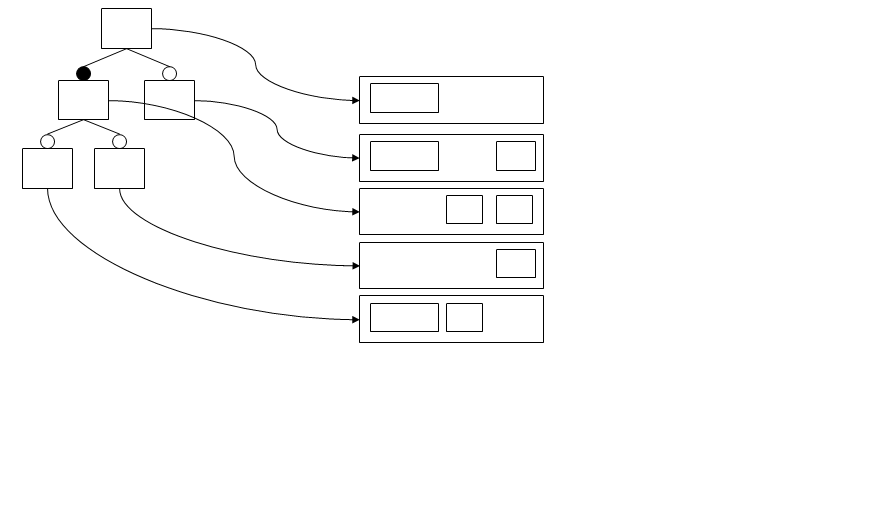
\includegraphics[height=0.8\textheight]{feature_komposition1}}
		\only<2| handout:0>{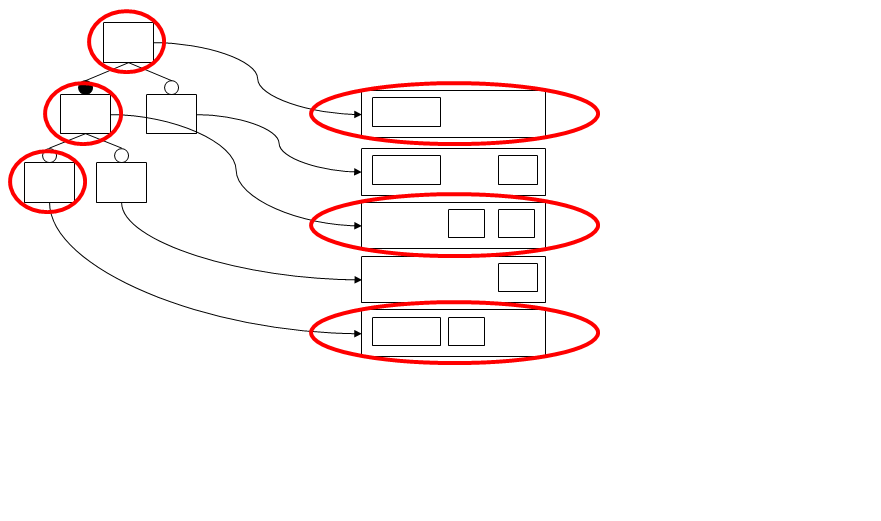
\includegraphics[height=0.8\textheight]{feature_komposition2}}
		\only<3| handout:0>{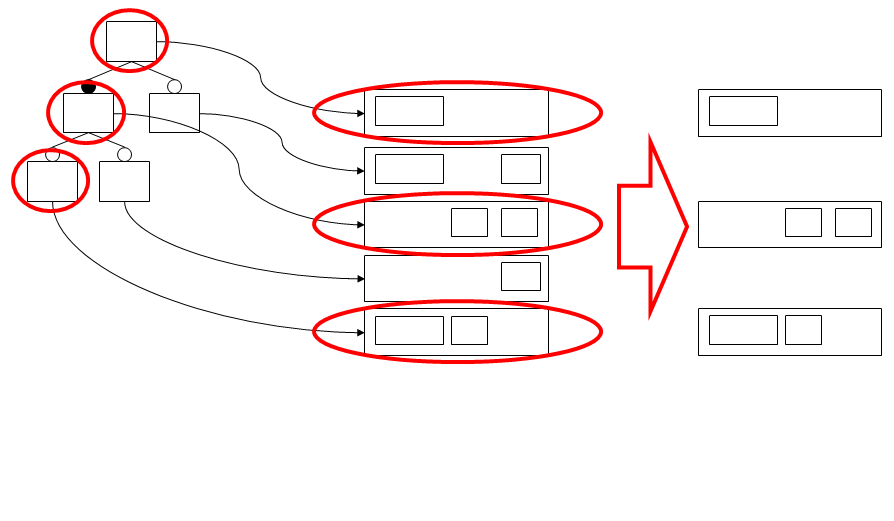
\includegraphics[height=0.8\textheight]{feature_komposition3}}
		\only<4>{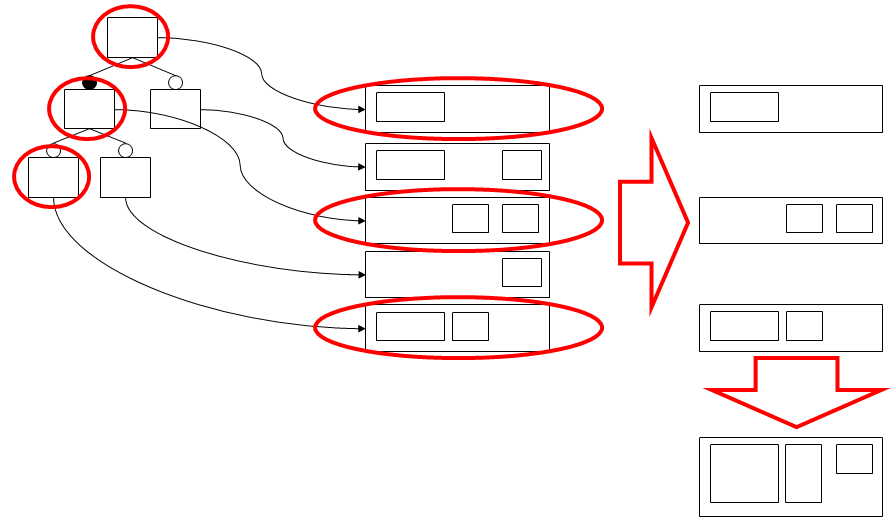
\includegraphics[height=0.8\textheight]{feature_komposition4}}
	\end{center}
\end{frame}

\begin{frame}{Practical Organization of Feature Modules}
	\begin{mycolumns}[widths={70,30},animation=none]
		\myexampletight{}{
			\centering
			\pic[width=1.0\linewidth]{fop-directories-fide}
		}
	\mynextcolumn
		\mynote{}{
			\begin{itemize}
				\item In most FOP tools, feature modules are represented by (nested) file-system directories
				\item Classes and their refinements are stored in files inside the corresponding containment hierarchies
			\end{itemize}
		}
	\end{mycolumns}
\end{frame}

\subsection{Principle of Uniformity}

\begin{frame}{Beyond Jak: Uniformity}
	\begin{mycolumns}[widths={35,65},animation=none]
		\mynote{Motivation}{
			\begin{itemize}
				\item Software does not only consist of Java source code, but also other programming languages, build scripts, documentation, models, etc.
				\item All software artifacts must be refined 
				\item Integration of different artifacts in collaborations
			\end{itemize}
		}
	\mynextcolumn
		\mydefinition{Idea}{
			\begin{itemize}
				\item Each feature is represented by a containment hierarchy: 
				\begin{itemize}
					\item Directory structure organizes the feature's artifacts.
					\item At the file level, there may be heterogeneous artifacts.
				\end{itemize}
				\item Composing features means composing containment hierarchies and, to this end, composing corresponding artifacts recursively by name and type
				\item For each artifact type, a different implementation of the composition operator ``$\bullet$'' has to be provided in AHEAD (just like the Jak-composition tool)
			\end{itemize}
		}
	\end{mycolumns}
\end{frame}

\begin{frame}{Beyond Jak: Uniformity}
	\myexampletight{}{
		\centering
		\pic[width=1.0\linewidth]{composition_dir}
	}
\end{frame}

\begin{frame}{FeatureHouse: A Model and Framework for FOP}
	\begin{mycolumns}[widths={50,50},animation=none]
		\mydefinition{Goal}{
			\emph{Language-independent model and tool chain} to enhance given languages rapidly with support for feature-oriented programming
		}
		\mydefinition{Assumption}{
			\begin{itemize}
				\item A feature may be represented as tree, known as \emph{Feature Structure Tree (FST)}
				\item Example; Java: Packages, Classes, Methods and Fields 
			\end{itemize}
		}
	\mynextcolumn
		\mydefinition{Idea}{
			\begin{itemize}
				\item Composition = Superimposition of FSTs (i.e., recursively superimpose nodes of FST, starting with the root node)
				\item Inner nodes: Can be safely superimposed if they are identical (superimposed parents and same name), or added if non-identical
				\item Leaf nodes: Type-specific resolution of conflicts
			\end{itemize}
		}	
	\end{mycolumns}
\end{frame}

\begin{frame}{FeatureHouse: Overview}
	\myexampletight{}{
		\centering
		\pic[width=0.85\linewidth]{featurehouse}
	}
\end{frame}

\begin{frame}{FeatureHouse: Composition}
	\myexampletight{}{
		\centering
		\pic[width=0.77\linewidth]{featurehouse_composition}
	}
\end{frame}

\begin{frame}[fragile]{Example: Java Support in FeatureHouse}
	\begin{mycolumns}[widths={60,40},animation=none]
{\small
\begin{codetight}{}
class Edge {
	private Node a, b;
	void print() {
		System.out.print("Edge between " + a + " and " + b);
	}
}
\end{codetight}
\begin{codetight}{}
class Edge {
	private Node start;
	void print() {
		original();
		System.out.print(" directed from " + start);
	}
}
\end{codetight}
\begin{codetight}{}
class Edge {
	private Weight weight;
	void print() {
		original();
		System.out.print(" weighted with " + weight);
	}
}
\end{codetight}
}
	\mynextcolumn
		\mynote{Differences compared to Jak}{
			\begin{itemize}
				\item No explicit keyword refines 
				\item Calling the method from previous refinement using keyword original
			\end{itemize}
		}
	\end{mycolumns}
\end{frame}

\subsection{Discussion}

\begin{frame}{Discussion}
	\begin{mycolumns}[widths={50,50},animation=none]
		\mynote{Advantages}{
			\begin{itemize}
				\item Easy to use language-based mechanism, requires only minimal language extensions.
				\item Conceptually uniformly applicable to code and noncode artifacts.
				\item Separation of (possibly crosscutting) feature code into distinct feature modules.
				\item Little preplanning required due to mixin-based extension mechanism.
				\item Direct feature traceability from a feature to its implementation in a feature module.
			\end{itemize}
		}
	\mynextcolumn
		\mynote{Disadvantages}{
			\begin{itemize}
				\item Requires adoption of a language extension and composition tools.
				\item Tools need to be constructed for every language (although with the help of a framework).
				\item Only academic tools so far, little experience in practice.
				\item Granularity restricted to method-level (or other named structural entities).
			\end{itemize}
		}
	\end{mycolumns}
\end{frame}



\lessonslearned{
	\item TODO
}{
	\item Batory et al.: Scaling Step-Wise Refinement. IEEE Transactions on Software Engineering, 30(6), 2004.
	\item Apel et al.: Language-Independent and Automated Software Composition: The FeatureHouse Experience. IEEE TSE, 39(1), 2013.
	\item \fospl, Chapter 6.1
	\item \featureide, Part 4
}{
	\item Why is class refinement in FOP different from inheritance in OOP, although it looks very similar?
	\item To some extent, FOP can be considered as static counterpart to the Decorator design pattern in OOP. Why?
	\item Consider the composition operator in FOP and the merge operator of traditional version control systems. Which are the major differences?
	\item In which sense does FOP violate the classical principles of information hiding and encapsulation of OPOP? What are the consequences?
	\item What might be the reasons that FOP has not yet been widely adopted in practice?
}

\sectionend

\section{Aspect-Oriented Programming}

\subsection{Motivation}

\begin{frame}{Recap: Motivation}
	\begin{mycolumns}[widths={50,50},animation=none]
		\myexampletight{Modularization of Cross-Cutting Concerns}{
			\centering
			\pic[width=1.0\linewidth]{aop-motivation-1}
		}
		\myexample{Feature Traceability}{
			find feature 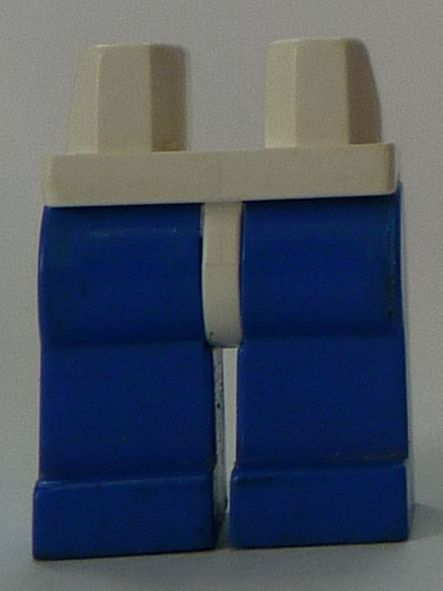
\includegraphics[width=.15\linewidth]{pants-blue} in product 
\includegraphics[width=.15\linewidth]{230}
		}
	\mynextcolumn
		\myexampletight{Flexible Extension / Minimal Preplanning}{
			\centering
			\pic[width=1.0\linewidth]{aop-motivation-2}
		}
		
		~
		
		\mynote{}{
			Achieving all this requires novel implementation techniques that overcome the limitations of classical object-oriented paradigms.
		}
	\end{mycolumns}
\end{frame}

\subsection{Aspects and Aspect Weaving}

\begin{frame}{Aspects and Aspect Weaving}
	\begin{mycolumns}[widths={50,50},animation=none]
		\mydefinition{Aspect \mysource{\fospl\mypages{143--145}}}{
			An aspect encapsulates the implementation of a crosscutting concern.
		}
		\mydefinition{Aspect Weaving \mysource{\fospl\mypages{143--145}}}{
			An aspect weaver merges the separate aspects of a program and the base program at user-selected program locations.
		}
		\mynote{}{
			\begin{itemize}
				\item Localizing a crosscutting concern within one code unit eliminates code scattering and tangling.
				\item An aspect can affect multiple other concerns with one piece of code, thereby avoiding code replication.
			\end{itemize}
		}
	\mynextcolumn
		\myexampletight{}{
			\centering
			\pic[width=1.0\linewidth]{aspect-weaving}
		}
	\end{mycolumns}
\end{frame}

\begin{frame}{Aspects and Aspect Weaving in Java: AspectJ}
	\begin{mycolumns}[widths={50,50},animation=none]
		\mydefinition{}{
			AspectJ is an aspect-oriented language extension of Java.
			\begin{itemize}
				\item Base program is written in Java (i.e., components = classes)
				\item Aspects are written in Java but typically include a multitute of new language constructs introduced by AspectJ
				\item Aspect weaver (aka.\ AspectJ Compiler) follows a compile-time binding approach (though certain decisions are made at runtime, s.\ later).
			\end{itemize}
		}
		\mynote{}{
			AspectJ is the most popular and widely used aspect-oriented language, all examples in this lecture will be given in AspectJ.
		}
	\mynextcolumn
		\myexampletight{}{
			\centering
			\pic[width=1.0\linewidth]{aspect-weaving}
		}
	\end{mycolumns}
\end{frame}

\subsection{Static vs. Dynamic Extensions}

\begin{frame}[fragile]{Static Extensions through Inter-Type Declarations}
	\begin{mycolumns}[widths={50,50},animation=none]
		\mydefinition{Inter-Type Declaration \mysource{\fospl\mypages{143--145}}}{
			An inter-type declaration injects a method, field, or interface from inside an aspect into an existing class or interface.
		}
		\mynote{Typical Usage}{
			Add field X / method Y to class Z
		}
	\mynextcolumn
\begin{codetight}{}
aspect Weighted {
	private int Edge.weight = 0;
	public void Edge.setWeight(int w) {
		weight = w;
	}
}
\end{codetight}
	\end{mycolumns}
\end{frame}

\begin{frame}{Dynamic Extensions through Join Points}
	\begin{mycolumns}[widths={50,50},animation=none]
		\mydefinition{Joint Point \mysource{\fospl\mypages{143--145}}}{
			A join point is an event in the execution of a program at which aspects can be woven into the program.
		}
		\mydefinition{Advice}{
			Code which is being executed when a join point matches. 
		}
		\mydefinition{Join-Points in AspectJ:}{
			\begin{itemize}
				\item Calling/executing a method/constructor
				\item Access to a field (read or write)
				\item Catching an Exception
				\item Execution of a Advice
				\item \ldots
			\end{itemize}
		}
	\mynextcolumn
		\myexampletight{}{
			\centering
			\pic[width=1.0\linewidth]{join_point_example}
		}
		
		~
		
		\mynote{Open Question}{			
			How to specify the join points an aspect (i.e., an advice) affects?
		}
	\end{mycolumns}
\end{frame}

\subsection{Quantification}

\begin{frame}[fragile]{Quantification through Pointcuts}
	\begin{mycolumns}[widths={50,50},animation=none]
		\mydefinition{Pointcut \mysource{\fospl\mypages{143--145}}}{
			A pointcut is a declarative specification of the join points that an aspect affects. It is a predicate that determines whether a given join point matches.
		}
		\mydefinition{Quantification \mysource{\fospl\mypages{143--145}}}{
			Quantification is the process of selecting multiple join points based on a declarative specification (that is, based on a pointcut).
		}
		\myexample{}{
			\begin{itemize}
				\item Execute Advice X whenever the method setWeight of class Edge is called
				\item Execute Advice Y whenever any field in class Edge is accessed
				\item Execute Advice Z whenever a public method is called anywhere in the system and the method initialize has been called beforehand
			\end{itemize}
		}
	\mynextcolumn
\begin{codetight}{Anonymous Pointcut}
aspect A1 {
	after() : execution(int MathUtil.twice(int)) {
		System.out.println("MathUtil.twice executed");
	}
}
\end{codetight}			
\begin{codetight}{Explicit Pointcut}
aspect A2 {
	pointcut executeTwice() : execution(int MathUtil.twice(int));
	after() : executeTwice() {
		System.out.println("MathUtil.twice executed");
	}
}
\end{codetight}			
	\end{mycolumns}
\end{frame}

\begin{frame}[fragile]{Quantification over other Join Points}
	\begin{mycolumns}[widths={50,50},animation=none]
\begin{codetight}{Call of a method}
aspect A1 {
	after() : call(int MathUtil.twice(int)) {
		System.out.println("MathUtil.twice called");
	}
}
\end{codetight}
	\mynextcolumn
\begin{codetight}{Base Program}
class Test {
	public static void main(String[] args) {
		MathUtil u = new MathUtil();
		int i = 2;
		i = u.twice(i);
		i = u.twice(i);
		System.out.println(i);
	}
}

class MathUtil {
	public int twice(int i) {
		return i * 2;
	}
}
\end{codetight}	
	\end{mycolumns}
\end{frame}

\begin{frame}[fragile]{Quantification over other Join Points}
	\begin{mycolumns}[widths={50,50},animation=none]
\begin{codetight}{Call of a method}
aspect A1 {
	after() : call(int MathUtil.twice(int)) {
		System.out.println("MathUtil.twice called");
	}
}
\end{codetight}
\begin{codetight}{Constructor call}
aspect A1 {
	after() : call(MathUtil.new()) {
		System.out.println("MathUtil created");
	}
}
\end{codetight}
	\mynextcolumn
\begin{codetight}{Base Program}
class Test {
	public static void main(String[] args) {
		MathUtil u = new MathUtil();
		int i = 2;
		i = u.twice(i);
		i = u.twice(i);
		System.out.println(i);
	}
}

class MathUtil {
	public int twice(int i) {
		return i * 2;
	}
}
\end{codetight}	
	\end{mycolumns}
\end{frame}

\begin{frame}[fragile]{Quantification over other Join Points}
	\begin{mycolumns}[widths={50,50},animation=none]
\begin{codetight}{Call of a method}
aspect A1 {
	after() : call(int MathUtil.twice(int)) {
		System.out.println("MathUtil.twice called");
	}
}
\end{codetight}
\begin{codetight}{Constructor call}
aspect A1 {
	after() : call(MathUtil.new()) {
		System.out.println("MathUtil created");
	}
}
\end{codetight}
		\mynote{And many more}{
			\begin{itemize}
				\item get: field access (read)
				\item set: field access (write)
				\item etc.
			\end{itemize}
		}
	\mynextcolumn
\begin{codetight}{Base Program}
class Test {
	public static void main(String[] args) {
		MathUtil u = new MathUtil();
		int i = 2;
		i = u.twice(i);
		i = u.twice(i);
		System.out.println(i);
	}
}

class MathUtil {
	public int twice(int i) {
		return i * 2;
	}
}
\end{codetight}	
	\end{mycolumns}
\end{frame}

\begin{frame}[fragile]{Further Quantification Options}
	\begin{mycolumns}[widths={70,30},animation=none]
\begin{codetight}{Pointcuts with ``Wildcards''}
aspect A1 {
	pointcut P1() : execution(int MathUtil.twice(int));
	pointcut P2() : execution(* MathUtil.twice(int));
	pointcut P3() : execution(int MathUtil.twice(*));
	pointcut P4() : execution(int *.twice(int));
	pointcut P5() : execution(int MathUtil.twice(..));
	pointcut P6() : execution(int MathUtil.twice(int));
}
\end{codetight}
\begin{codetight}{Logial Connections of Pointcuts}
aspect A1 {
	pointcut P2(): call(* MathUtil.*(..)) && !call(* MathUtil.twice(*));
	pointcut P3(): execution(* MathUtil.twice(..)) && args(int);
}
\end{codetight}
	\mynextcolumn
		\mynote{Wildcard Symbols}{
			\begin{itemize}
				\item [*] Exactly one value
				\item [..] Arbitrary many values
				\item [+] Class or any subclass
			\end{itemize}
		}		
		\mynote{Logical Connectors}{
			Pointcuts can be connected by usual logical operators \&\&, $\mid\mid$, and !
		}
	\end{mycolumns}
\end{frame}

\subsection{Executing Additional Code}

\begin{frame}[fragile]{Advice}
	\begin{mycolumns}[widths={38,62},animation=none]
		\mynote{}{
			\begin{itemize}
				\item Additional code before, after or instead of the join point: before, after, around
				\item Around-Advice allows to continue the original join point using the keyword proceed
				\item Keyword \emph{proceed} corresponds to keyword \emph{original/super} in FOP
			\end{itemize}
		}
	\mynextcolumn
{\small
\begin{codetight}{}
public class Test2 {
	void foo() {
		System.out.println("foo() executed");
	}
}
aspect AdviceTest {
	before(): execution(void Test2.foo()) {
		System.out.println("before foo()");
	}
	after(): execution(void Test2.foo()) {
		System.out.println("after foo()");
	}
	void around(): execution(void Test2.foo()) {
		System.out.println("around begin");
		proceed();
		System.out.println("around end");
	}
	after() returning (): execution(void Test2.foo()) {
		System.out.println("after returning from foo()");
	}
	after() throwing (RuntimeException e): execution(void Test2.foo()) {
		System.out.println("after foo() throwing "+e);
	}
}
\end{codetight}
}
	\end{mycolumns}
\end{frame}

\begin{frame}[fragile]{thisJoinPoint}
	\begin{mycolumns}[widths={30,70},animation=none]
		\mynote{}{
			In an advice, \emph{thisJoinPoint} can be used to get more information about the current join point.
		}
	\mynextcolumn
\begin{codetight}{}
aspect A1 {
	after() : call(int MathUtil.twice(int)) {
		System.out.println(thisJoinPoint);
		System.out.println(thisJoinPoint.getSignature());
		System.out.println(thisJoinPoint.getKind());
		System.out.println(thisJoinPoint.getSourceLocation());
	}
}
\end{codetight}
\begin{codetight}{Output}
call(int MathUtil.twice(int))
int MathUtil.twice(int)
method-call
Test.java:5
\end{codetight}
	\end{mycolumns}
\end{frame}

\begin{frame}[fragile]{Parameterized Pointcuts}
	\begin{mycolumns}[widths={60,40},animation=none]
\begin{codetight}{}
aspect A1 {
	pointcut execTwice(int value) :
			execution(int MathUtil.twice(int)) && args(value);
	after(int value) : execTwice(value) {
		System.out.println("MathUtil.twice executed with parameter " + value);
	}
}
\end{codetight}
\begin{codetight}{}
aspect A1 {
	after(int value) : execution(int MathUtil.twice(int)) && args(value) {
		System.out.println("MathUtil.twice executed with parameter " + value);
	}
}
\end{codetight}
	\mynextcolumn
\begin{codetight}{Base Program}
class Test {
	public static void main(String[] args) {
		MathUtil u = new MathUtil();
		int i = 2;
		i = u.twice(i);
		i = u.twice(i);
		System.out.println(i);
	}
}

class MathUtil {
	public int twice(int i) {
		return i * 2;
	}
}
\end{codetight}	
	\end{mycolumns}
\end{frame}

\begin{frame}[fragile]{Pointcuts this and target}
	\begin{mycolumns}[widths={50,50},animation=none]
		\mynote{}{
			\begin{itemize}
				\item \emph{execution}: this and target capture the object on which the method is called
				\item \emph{call, set, and get}: this captures the object that calls the method or accesses the field; 
																	target captures the object on which the method is called or the field is accessed.
			\end{itemize}
		}
	\mynextcolumn
\begin{codetight}{}
aspect A1 {
	pointcut P1(Main s, MathUtil t): 
		call(* MathUtil.twice(*)) 
		&& this(s) 
		&& target(t);
}
\end{codetight}	
	\end{mycolumns}
\end{frame}

\begin{frame}[fragile]{Order Matters: Aspect Precendence}
	\begin{mycolumns}[widths={50,50},animation=none]
		\mynote{}{
			Order in which aspect weaver process the aspects may be relevant when multiple aspects extend the same join point.
		}
		\myexample{Example}{
			\begin{itemize}
				\item 1st aspect implements synchronization with around advice
				\item 2nd aspect implements logging with after-advice on the same join point
				\item Depending on the order of weaving, the logging code will be synchronized or not
			\end{itemize}
		}
	\mynextcolumn
\begin{codetight}{Explicit definition using declare precedence}
aspect DoubleWeight {
	declare precedence : *, Weight, DoubleWeight;
	[...]
}
\end{codetight}	
	\end{mycolumns}
\end{frame}

\begin{frame}{Aspect Weaving: Behind the Scenes }
	\begin{mycolumns}[widths={50,50},animation=none]
		\mydefinition{Weaving in AspectJ (Conceptually)}{
			\begin{itemize}
				\item Inter-type declarations are added to respective classes
				\item Each advice is converted into a method
				\item Pointcuts: Add method call from the join points to the advice
				\item Dynamic extensions: Insert source code at all potential join points that checks dynamic conditions and, if conditions hold, calls the advice method.
			\end{itemize}
		}
	\mynextcolumn
		\mynote{Weaving in AspectJ (Technically)}{
			AspectJ Compiler; conceptual effect is only visible in Bytecode
		}
		\mynote{Other Options}{
			\begin{itemize}
				\item Source transformation: Base Program + Aspects $\rightarrow$ Java (s. FOP/Jak).
				\item Evaluation at runtime: Meta-Object Protocol, interpreted languages, ...
			\end{itemize}
		}
	\end{mycolumns}
\end{frame}

\subsection{Aspects for Product Lines}

\begin{frame}[fragile]{Typical (Traditional) Aspects}
	\begin{itemize}
		\item Logging, Tracing, Profiling
		\item Adding identical code to a large number of methods
	\end{itemize}
\begin{codetight}{Record time to execute my public methods}
aspect Profiler {   
    Object around() : execution(public * com.company..*.* (..)) {
        long start = System.currentTimeMillis();
        try {
            return proceed();
        } finally {
            long end = System.currentTimeMillis();
            printDuration(start, end, 
                thisJoinPoint.getSignature());
        }
    }
    // implement recordTime...
}
\end{codetight}	
\end{frame}

\begin{frame}[fragile]{Aspects for Product Lines}
	\begin{mycolumns}[widths={45,55},animation=none]
		\mydefinition{Basic Idea}{
			\begin{itemize}
				\item Implement one aspect per feature.
				\item Feature selection determines the aspects which are included in the weaving process.
			\end{itemize}
		}
		\mynote{}{
			\begin{itemize}
				\item Aspects encapsulate changes to be made to existing classes. 
				\item However, aspects do not encapsulate new classes introduced by a feature (only nested classes within an aspect)\\
					\emph{$\Rightarrow$ Gives rise to a combination of FOP and AOP.}
			\end{itemize}
		}
	\mynextcolumn
\begin{codetight}{A Color Feature for Graphs}
aspect ColorFeature {
	Color Node.color = new Color();
	
	before(Node n): execution(void print()) && this(n) {
		Color.setDisplayColor(n.color);
	}
	
	static class Color {
		...
	}
}
\end{codetight}	
	\end{mycolumns}
\end{frame}

\subsection{Discussion}

\begin{frame}{Controversial: Obliviousness and Fragile-Pointcut Problem}
	\begin{mycolumns}[widths={45,55},animation=none]
		\mydefinition{Principle of Obliviousness}{
			Base program is (deliberately) supposed to be oblivious wrt.\ the aspects that ``hook into'' the system:
			\begin{itemize}
				\item Base program developers implement their concerns as if there were no aspects.
				\item Aspect programmers extend the base program.
			\end{itemize}
		}
	\mynextcolumn
		\mydefinition{Fragile-Pointcut Problem}{
			Base program may be modified such that the set of join points changes in an undesired way:
			\begin{itemize}
				\item Join points may be removed accidentally 
				\item Join points may be captured by aspects accidentally
			\end{itemize}
		}
		\myexampletight{}{
			Example: Renaming a method that is (is not) to be advised
		}
	\end{mycolumns}
	\mynote{Obliviousness worsens the fragile-pointcut problem}{
		Because the base programmer does not know about aspects, it is more likely that changes may break aspect bindings and that nobody notices that.
	}
\end{frame}

\begin{frame}{Discussion}
	\begin{mycolumns}[widths={50,50},animation=none]
		\mynote{Advantages}{
			\begin{itemize}
				\item Separation of (possibly crosscutting) feature code into distinct aspects.
				\item Direct feature traceability from feature to its implementation in an aspect.
				\item Little or no preplanning effort required.
				\item Fine-grained variability driven by the join-point model of the aspect-oriented language.
			\end{itemize}
		}
	\mynextcolumn
		\mynote{Disadvantages}{
			\begin{itemize}
				\item Requires adoption of a rather complex extension mechanism (new language and paradigm).
				\item No unifying theory like no language-independent framework.
				\item Program evolution and maintenance affected by fragile-pointcut problem.
			\end{itemize}
		}
	\end{mycolumns}
\end{frame}

\lessonslearned{
	\item TODO
}{
  \item Kiczales et al: Aspect-oriented programming. Proc. Europ. Conf. Object-Oriented Programming. 1997
	\item Filman et al.: Aspect-oriented software development. Addison-Wesley. 2005
	\item \fospl, Chapter 6.2
}{
	\item Which features particularly benefit from the concept of quantification?
	\item What similarities and differences do you see between FOP and AOP?
	\item To what extent can FOP and AOP be combined profitably?
}

\mode<beamer>{
	\begin{frame}{\inserttitle}
		\lectureseriesoverview
	\end{frame}

	\contentoverview
}


\end{document}
